\chapter{Recognition on SpiNNaker}
\label{cha:rsp}

\section{Moving to spiking neurons}
\label{sec:msn}
\textcolor{red}{Mathematical approach.Need to work hard on.}

It remains a challenge to map the weights of a traditional artificial neural network to a spiking neural network. 
There are attempts to estimate the rate of Leaky integrate-and-fire (LIF) neurons with Poisson input spike trains~\cite{la2008response}. 
For the model illustrated above, there are two types of synaptic connection: one-to-one connections in the retina layer and N-to-one connections in all the convolutional layers (the pooling layer is also included). 
For the retina layer, 1) the problem is: what is the connection weight between two single LIF neurons to make a post-synaptic neuron fire whenever the pre-synaptic neuron generates a spike? 
While for the convolutional neurons, 2) given the input spike rates, LIF neuron parameters and the output spiking rate, what are the corresponding weights between the two layers?
\textcolor{blue}{In terms of the main goals of the report, the detailed mathematical reasoning will be demonstrated in the paper which will be submitted in November. 
A lot of work to be done here.}


\section{Recorded data test}
\label{sec:rdt}
New experiment to work on.

New tool need to be fixed (Spike Source Array), and maybe new ways of reloading.

\section{Real-time test}
\label{sec:rtt}
We implemented the prototype of the neural gesture recognition system on SpiNNaker. 
The input retina layer consists of 128$\times$128 neurons; 
each Gabor filter has 112$\times$112 valid neurons, since the kernel size is 17$\times$17; 
each pooling layer is as big as 36$\times$36, convolving with five template kernels (21$\times$21); 
thus, the recognition populations are 16$\times$16 neurons each. Altogether 74,320 neurons and 15,216,512 synapses use up to 19 chips on a 48-node board.

Figure~\ref{fig:live} shows snapshots of the real time gesture recognition system. Figure~\ref{fig:live1} is a snapshot of the Gabor filter layer, where Figure~\ref{fig:live2} shows the integration of all the pooled populations, and the active neurons in the visualizer in Figure~\ref{fig:live3} are pointing out the position of the recognized pattern (One finger). All the videos can be found on Youtube\footnote{\url{
http://youtu.be/PvJy6RKAJhw?list=PLxZ1W-Upr3eoQuLxq87qpUL-CwSphtEBJ, http://youtu.be/FZJshPCJ1pg?list=PLxZ1W-Upr3eoQuLxq87qpUL-CwSphtEBJ, http://youtu.be/yxN90aGGKvg?list=PLxZ1W-Upr3eoQuLxq87qpUL-CwSphtEBJ}}.

%\begin{figure}
%\centering
%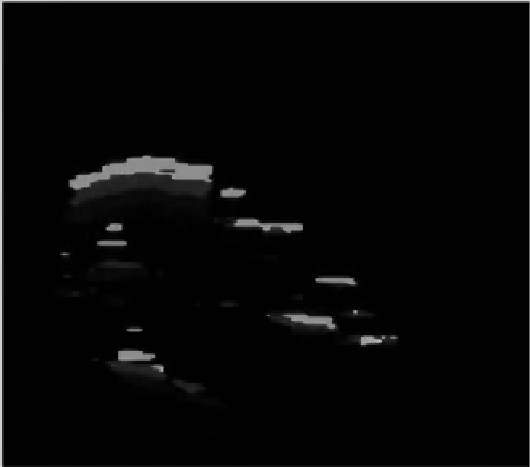
\includegraphics[width=0.7\textwidth]{pics/live1.png}
%\caption{Outline of the platform}
%\label{fig:live1}
%\end{figure}
%
%\begin{figure}
%\centering
%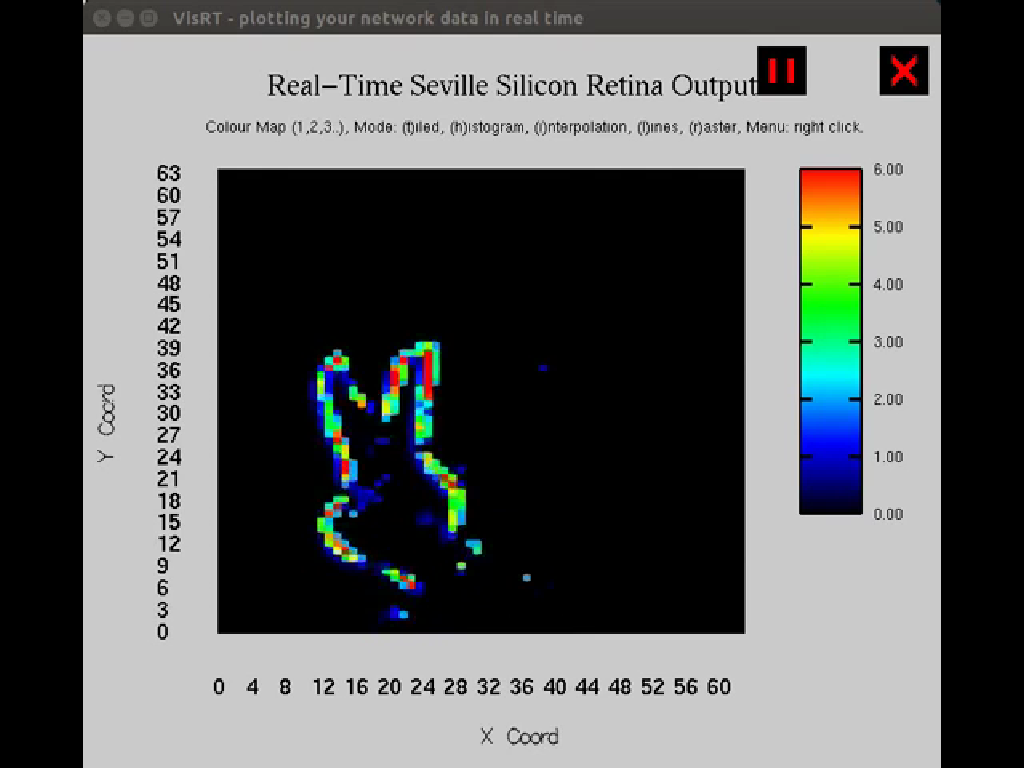
\includegraphics[width=0.7\textwidth]{pics/live2.png}
%\caption{Outline of the platform}
%\label{fig:live2}
%\end{figure}
%
%\begin{figure}
%\centering
%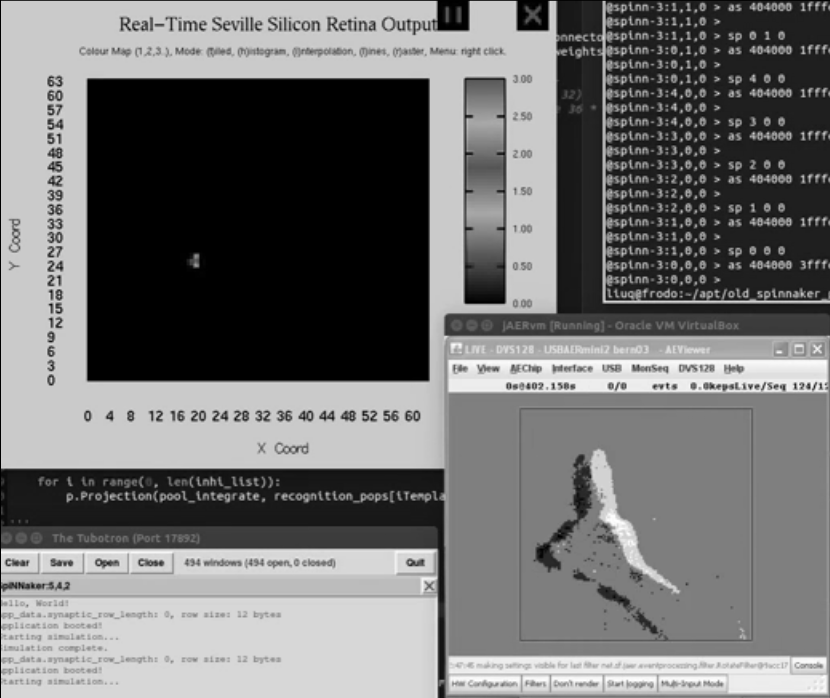
\includegraphics[width=0.7\textwidth]{pics/live.png}
%\caption{Outline of the platform}
%\label{fig:live3}
%\end{figure}

%ctlr + T and ctlr + U
\begin{figure}
\centering
	\begin{subfigure}[t]{0.42\textwidth}
		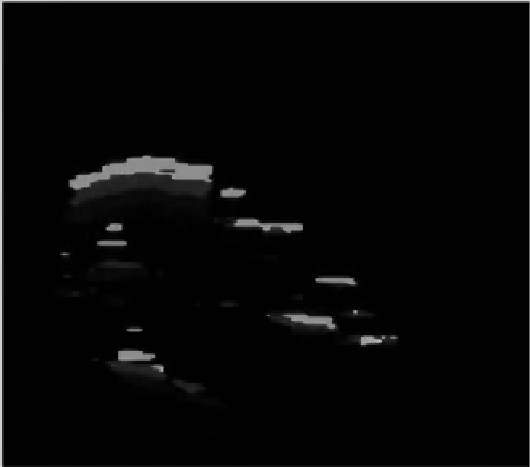
\includegraphics[width=\textwidth]{pics/live1.png}
	    \caption{Outline of the platform}
	    \label{fig:live1}
	\end{subfigure}
	\begin{subfigure}[t]{0.42\textwidth}
		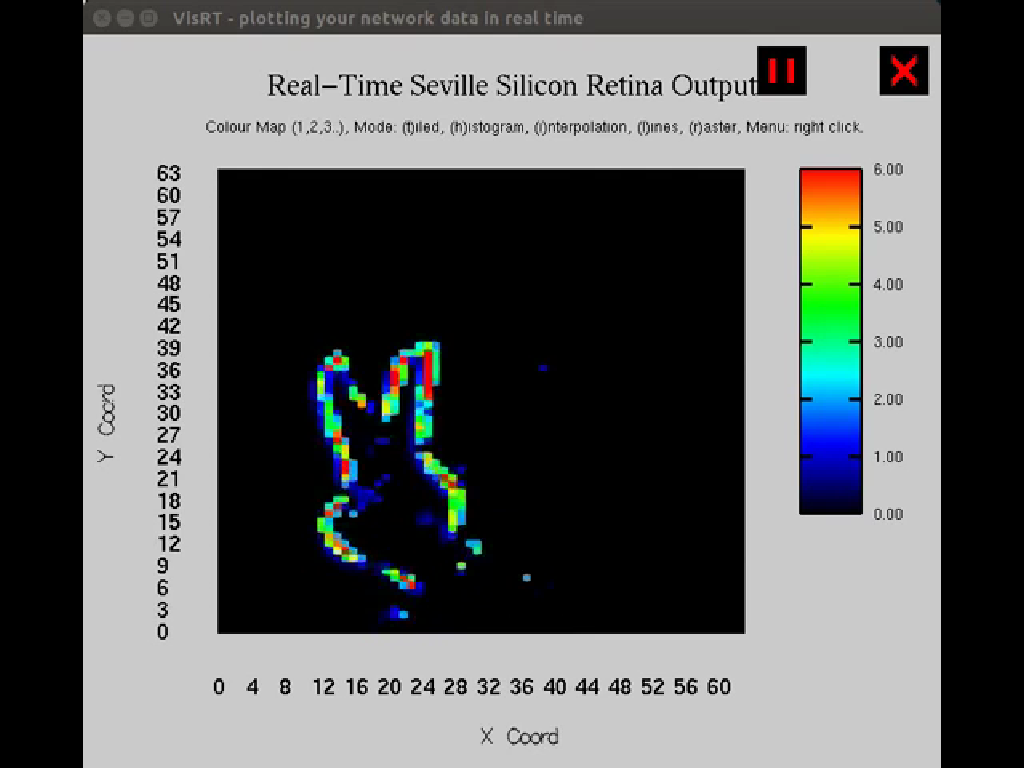
\includegraphics[width=\textwidth]{pics/live2.png}
		\caption{Picture of the hardware platform}
	    \label{fig:live2}
	\end{subfigure}
	\\
	\begin{subfigure}[t]{0.84\textwidth}
		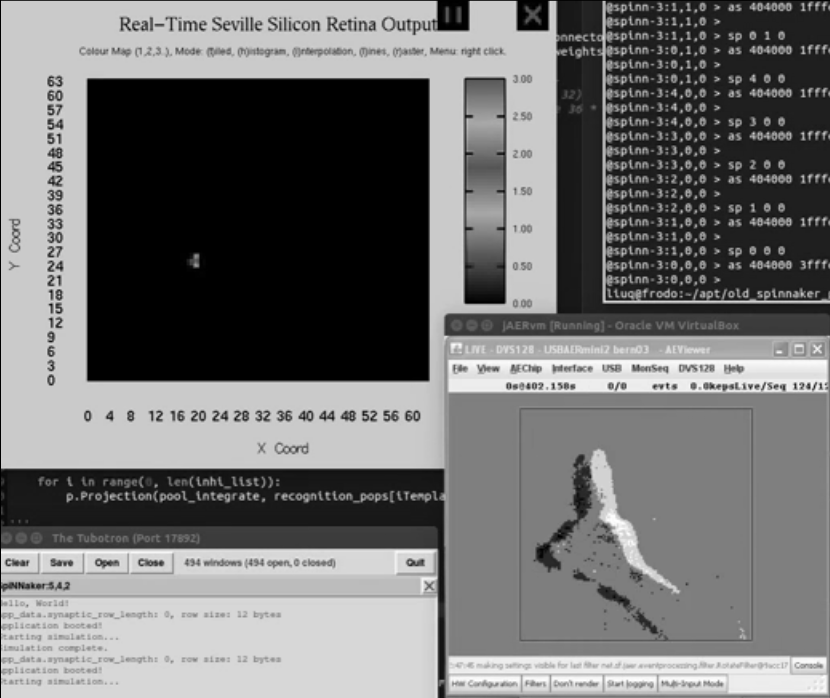
\includegraphics[width=\textwidth]{pics/live.png}
		\caption{Picture of the hardware platform}
	    \label{fig:live3}
	\end{subfigure}	

\caption{Snapshots of the real-time gesture recognition system on SpiNNaker.
}
\label{fig:live}
\end{figure}
